\section{Résultats}
\label{sec:resultats}

\subsection{Première expérience}

Les résultats de la première expérience sont montrés dans la \figref{renaming}. Tout d'abord, le nombre de renommage varie beaucoup entre les projets. Par exemple, Jenkins a au plus $10\%$ de ses fichiers renommés dans la pire période alors que PHPUnit a deux périodes à plus de $50\%$. Le nombre de renommages varie aussi en fonction des périodes, par exemple dans PHPUnit la période $3.6 - 3.7$ a moins de $5\%$ de fichiers renommés alors que la période $3.7 - 4.0$ a presque $99\%$. En général, il y a beaucoup de périodes avec $0\%$ de fichiers renommés.\\

\begin{figure*}[h]
	\centering
	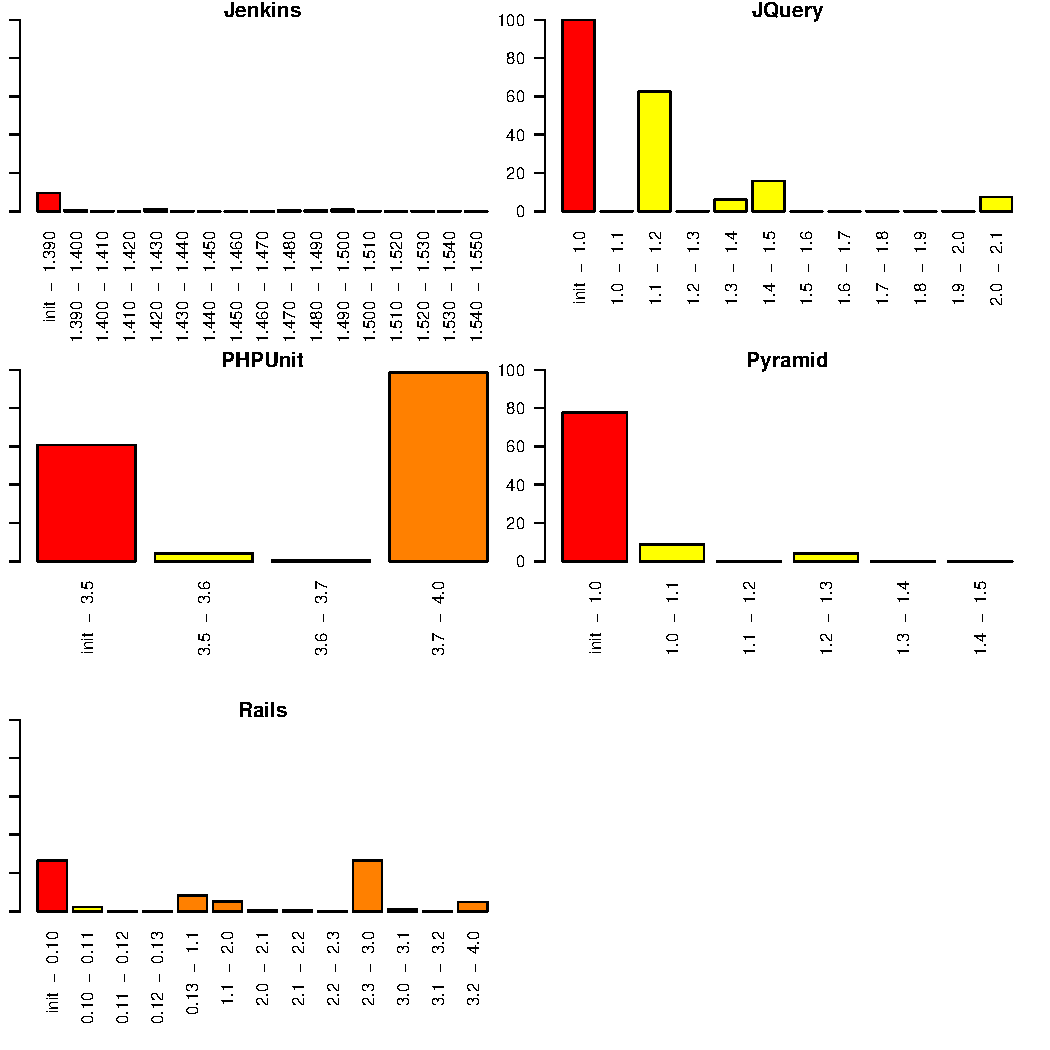
\includegraphics[width=0.85\linewidth,keepaspectratio]{data/figures/renaming.pdf}
	\caption{Pourcentage de fichiers renommés ($\%F_R$) dans chaque période de chaque projet de notre corpus. La période initiale est en rouge, les périodes majeures en orange et les périodes mineures en jaune. (resp. gris foncé, gris et gris clair sur une version papier du rapport)}
	\label{fig:renaming}
\end{figure*}

Par rapport à la localisation de ces renommages, la période initiale semble la plus prolifique. En général, elle contient le plus grand nombre de fichiers renommés (sauf pour PHPUnit). Les périodes de développement sont plus susceptibles d'avoir des renommages que les périodes de maintenance. Ainsi, les $5$ projets sont quasiment à $0\%$ de fichiers renommés dans les périodes de maintenance. Certaines périodes de développement peuvent contenir beaucoup de renommages. Les résultats montrent que les releases majeures sont souvent les pires périodes de développement en nombre de fichiers renommés: C'est le cas pour PHPUnit et Rails alors que Jenkins et Pyramid ne contiennent pas de releases majeures.\\

%Le détail des résultats obtenus par notre outil de détection de renommage sont montrés dans les tables en annexes \tabref{jenkins}, \tabref{jquery}, \tabref{phpunit}, \tabref{pyramid} et %\tabref{rails}. Ces tables mettent en avant les valeurs suivantes:\\

%\begin{itemize}
%\item \emph{Nombre de fichiers ($\#F$):} nombre de fichiers dans le projet à la dernière version de la période..
%\item \emph{Nombre de fichiers actifs ($\#AF$):} nombre de fichiers créés, suprimés, copiés ou renommés durant la période et présents à la dernière version de la période.
%\item \emph{Pourcentage de fichiers actifs ($\%AF$):} $\%AF = \frac{\#AF}{\#F}$.
%\item \emph{Nombre de fichiers actifs renommés ($\#AF_{r}$):} nombre de fichiers actifs qui ont étés renommés.
%\item \emph{Pourcentage de fichiers renommés ($\%F_{R}$):} $\%F_{R} = \frac{\#AF_{R}}{\#F}$.
%\item \emph{Pourcentage de fichiers actifs renommés ($\%AF_{R}$):} $\%AF_{R} = \frac{\#AF_{R}}{\#AF}$.
%\end{itemize}

En ce qui concerne le pourcentage de fichiers \textbf{actifs} renommés ($\%AF_R$) dans les périodes de nos projets, la \figref{renaming2} présente nos résultats. Nous pouvons remarquer que le taux de fichiers renommés ne change pas ou augmente légèrement pour Jenkins par exemple. Etant donné que $\%AF_R \geq \%F_R$ comme nous l'avons expliqué \secref{methodologie}, on en déduit qu'une grande partie des périodes, en tout cas les périodes qui ont un impact sur l'ensemble du projet, atteignent la totalité ou une grande partie (Jenkins) des fichiers du projet durant la période. \\

\begin{figure*}[h]
	\centering
	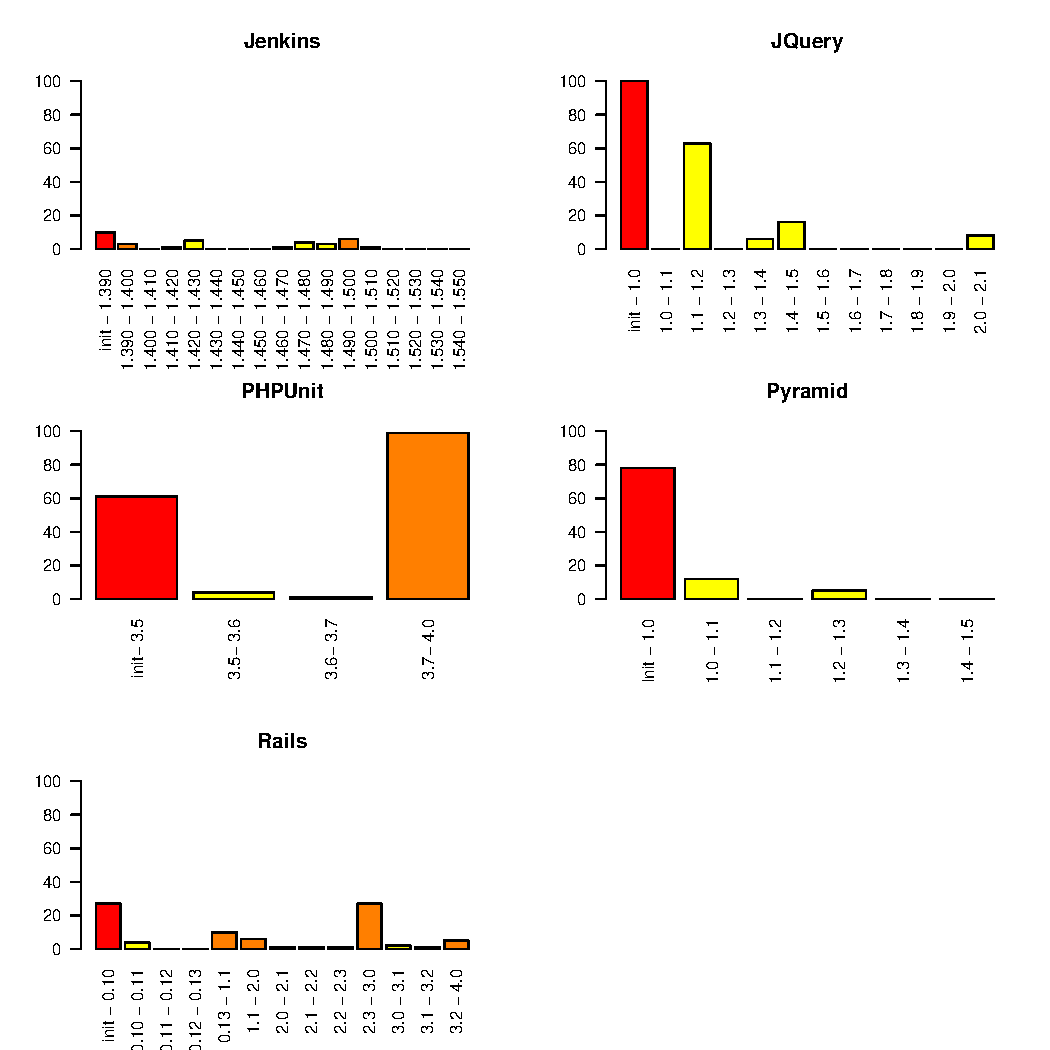
\includegraphics[width=0.85\linewidth,keepaspectratio]{data/figures/renaming2.pdf}
	\caption{Pourcentage de fichiers actifs renommés ($\%AF_R$) dans chaque période de chaque projet de notre corpus. La période initiale est en rouge, les périodes majeures en orange et les périodes mineures en jaune. (resp. gris foncé, gris et gris clair sur une version papier du rapport)}
	\label{fig:renaming2}
\end{figure*}

\subsection{Deuxième expérience}
Les résultats de notre deuxième expérience sont présentés dans la \tabref{spearman}. Ils montrent que le coefficient de corrélation de Spearman entre les métriques de procédés avec et sans détection de renommages dépend beaucoup de la période et de la métrique choisie. Les métriques de procédés ne sont pas affectées par le renommage dans les projets Jenkins, Rails et Pyramid. Ainsi, le coefficient de corrélation est proche de $1$ dans tous les cas. D'un autre côté, pour PHPUnit et JQuery les métriques peuvent être sévèrement impactées par le renommage. Pour JQuery, la métrique Code Churn n'est pas affectée par le renommage, mais NoD et NoC sont quant à eux significativement impactés. Pour PHPUnit, toutes les métriques sont affectées par le renommage. Sur ces deux derniers projets, la métrique la plus sensible aux renommages de fichiers est le nombre de développeurs (NoD). Sur ces deux derniers projets, la métrique la plus sensible aux renommages de fichiers est le nombre de développeurs (NoD).

Finalement, on peut noter que seules les périodes ayant eu un grand pourcentage de fichiers renommés ($\%F_R$) ont été impactées. On peut aussi noter que des métriques biaisées par le renommage ont été calculées dans des releases majeures et mineures.\\

Nous avons étudié manuellement les deux périodes qui ont affecté les valeurs des métriques de procédés (JQuery 1.1 - 1.2 et PHPUnit 3.7 - 4.0). Dans ces deux périodes, la structure générale du projet a été modifiée. Notamment, des renommages de dossiers à la racine ont été effectués. Par conséquent, un grand nombre de fichiers a été renommé de manière transitive. C'est une pratique courante dans le développement logiciel, donc le phénomène pourrait apparaitre dans n'importe quelle période ou projet. Il est intéressant de noter que dans ces deux périodes, les changements de structure ont été effectués en grande partie dans un seul commit proche de la fin de la période.\\
\newpage

\begin{table*}[h]
\centering
\csvreader[tabular=rcccc, table head=\toprule & & \multicolumn{3}{c}{Métriques de procédés}\\\cmidrule{3-5} Période & $\%F_R$ & CC & NoD & NoC\\\midrule, late after line=\\, late after last line=\\\bottomrule]{data/tables/correlations.csv}%
{1=\period,2=\fr,3=\churnall,4=\devall,5=\modificationsall}%
{\period & \fr & \churnall & \devall & \modificationsall}
\caption{La corrélation de coefficients de Spearman entre les valeurs des métriques de procédés avec et sans détection de renommage. Les coefficients moyen et faible sont affichés en gras.}
\label{tab:spearman}
\end{table*}

\subsection{Validations et limitations}

Notre étude fait l'hypothèse que les renommages détectés par Git sont corrects. Néanmoins, nous n'avons pas rencontré d'évaluation empirique de l'algorithme de détection de renommage de Git. Par conséquent nous ne sommes pas sur de la qualité de ses performances. Afin d'atténuer le risque de fausser notre étude, nous avons tiré au hasard $100$ renommages détectés par Git lors de notre expérimentation. Nous avons évalué manuellement chaque renommage de fichier pour vérifier si la détection était correcte.\\ 

Vérifier que la détection soit correcte consiste à s'assurer que le contenu du fichier avant et après renommage soit très similaire, et qu'aucun autre fichier ajouté dans la même version n'ait un contenu similaire. Cette analyse manuelle nous a révélé que  $100\%$ des renommages étaient correctement détectés. La précision, qui est définie par le nombre de renommages justes détectés par l'algorithme de Git divisé par le nombre de renommages détectés, est donc de $1$. Même si nous ne connaissons pas le rappel de notre analyse, c'est-à-dire le nombre de renommages justes détectés divisé par le nombre de renommages du projet (incluant ceux qui ne sont pas détectés), cette expérience montre que l'utilisation de Git dans la détection de renommage reste raisonnable. Nous n'avons pas analysé les faux négatifs, c'est à dire les vrais renommages de fichiers non détectés par Git. Cette analyse devrait se faire de manière manuelle afin de récupérer dans chaque \texttt{commit} la totalité des renommages. Ce qui n'est pas faisable compte tenu de la quantité considérable de données à analyser sur nos projets. De plus, cela ne pourrait que diminuer les coefficients de corrélation si nous l'avons sous-estimé et donc ne risquerait pas de fausser nos conclusions.\\  

Nous avons uniquement évalué l'effet du renommage sur trois métriques de procédés. L'effet du renommage pourrait être différent (et non prévisible) pour les autres métriques de procédés. Notre solution pour limiter ce risque était d'analyser les métriques de procédés les plus utilisées comme il est montré dans~\cite{radjenovic_software_2013}. Les autres métriques de procédés sont souvent basées sur ces trois métriques comme la métrique \emph{code ownership}~\cite{bird_dont_2011} ou \emph{module activity focus}~\cite{posnett_dual_2013}.\\

Pour la métrique NoD, nous n'avons pas appliqué un algorithme de fusion d'identités~\cite{goeminne_comparison_2013}. Il pourrait en résulter des valeurs incorrectes. Cependant, ce phénomène est susceptible d'arriver pour les deux calculs de métrique avec et sans le renommage, donc le risque qu'il invalide nos conclusions est faible.\\

Concernant notre conclusion sur la quantité de renommage, le corpus utilisé ne garantit pas qu'elle puisse être généralisée. En effet, nous avons uniquement utilisé des projets open-source, alors que les projets industriels sont connus pour être sensiblement différents. En ce qui concerne la validité sur les projets open-source, notre corpus est trop petit pour généraliser cette conclusion.\\
